\documentclass{BVP_AISC}

% AI and Security Convergence manuscript.
% Scientific results and methods reflect the frozen confirmatory study state
% described in the accompanying project records.

\received{}
\revised{}
\accepted{}
\published{}
\doi{}

\OAText{{\copyright} The Author(s) 2026. Published by BON VIEW PUBLISHING PTE. LTD. This is an open access article under the CC BY License (https://creativecommons.org/licenses/by/4.0/).}

\begin{document}

\arttype{Original Research Article}

\title{Construct Validity of Lexical Prompt-Injection Success Evaluators}

\author{Yixuan Wang$^{1,}$\thanks{\textbf{Corresponding author:} Yixuan Wang, Independent Researcher, Canada. Email: \email{wangharrison2009@gmail.com}}}

\affil{Independent Researcher, Canada, wangharrison2009@gmail.com}

\begin{abstract}
Prompt-injection studies often use lexical rules to decide whether an attack succeeds. Different rules measure different forms of attack compliance. This study tests the construct validity of two deterministic lexical evaluators against human judgments. S0 marks success when an exact attacker-controlled target appears anywhere in a model response. S2 marks success only when the same target begins at character position zero. We generated responses to 1,680 prompts across seven language tasks and three open-weight instruction-tuned models. After technical failures, the final population contained 4,993 usable responses. Two human annotators independently labeled a preregistered stratified sample of 800 responses. A third adjudicator reviewed disagreements, and the adjudication process resolved the remaining cases by consensus. Under a strict definition where only full attack compliance counted as success, weighted accuracy reached 81.100\% for S0 and 92.776\% for S2, a difference of 11.676 percentage points. When partial compliance also counted as success, the difference fell to 0.774 points. The strict S2 advantage was 23.034 points larger for generative and text-transformation tasks than for closed-label classification tasks. These results show lexical evaluators measure different forms of prompt-injection success. Evaluator choice should match the behavioral definition of attack success used in a security benchmark.
\end{abstract}

\begin{keywords}
prompt injection, construct validity, attack success rate, lexical evaluation, human annotation
\end{keywords}

\maketitle

\section{Introduction}\label{sec:intro}

Prompt injection is a security problem in large language model (LLM)-integrated applications in which attacker-controlled instructions are placed in an input or external content so that the model departs from the application's intended task. Systematic prompt-injection benchmarks have compared attacks and defenses across multiple models and tasks \cite{liu2024}, while large-scale adversarial efforts such as HackAPrompt have demonstrated the diversity of prompts that can induce unintended model behavior \cite{schulhoff2023}. Indirect prompt-injection benchmarks and agent-oriented evaluations have further shown that untrusted external content can influence LLM behavior in application settings \cite{yi2025,zhan2024}.

As the field has matured, evaluation methodology itself has become a security-research question. PIArena emphasizes the difficulty of comparing prompt-injection defenses across heterogeneous attacks, tasks, and benchmarks \cite{geng2026}, and recent work has shown that common research settings may not represent the range of real-world prompt-injection applications \cite{cui2026}. Other work has identified weaknesses in benchmark success metrics and stressed that apparently strong security conclusions can depend on evaluator design \cite{bhagwatkar2025}. These concerns motivate a narrower measurement question: even when the underlying model response is fixed, what security construct is represented by the automated rule used to declare an attack successful?

This question is especially important for lexical evaluators. They are deterministic, inexpensive, easy to audit, and highly reproducible, but a lexical match can represent several different behaviors. A model may reproduce an attacker-controlled target while discussing or rejecting it, may partially follow an injected instruction without completing the full objective, or may obey the legitimate task while incidentally mentioning target text. A recent indirect prompt-injection assessment explicitly found that deterministic and semantic judges assigned different rates of partial compliance, illustrating the sensitivity of attack-outcome measurement to evaluator semantics \cite{ying2026}.

We study two simple lexical evaluators for attacks whose objective is to begin the response with an exact attacker-controlled target and then complete the legitimate task. The first evaluator, S0, declares success if the exact target occurs anywhere in the raw response. The second, S2, declares success only if the exact target begins at character position zero. Because S2 success is structurally a subset of S0 success, S0's raw ASR cannot be lower than S2's by construction. We therefore do not treat the S0--S2 ASR ordering as empirical evidence. Instead, we test how each evaluator aligns with independently adjudicated human judgments of attack behavior.

The preregistered sole primary hypothesis (H1) predicted that S2 would agree more closely than S0 with human judgments of \texttt{FULL\_COMPLIANCE}. A second research question (RQ2) estimated how that difference changed when human success was defined leniently to include both full and partial compliance. A gated secondary hypothesis (H3) predicted that the strict S2-versus-S0 human-alignment advantage would be larger for generative/text-transformation tasks than for closed-label classification tasks. The results show a large S2 advantage under strict full-compliance judgments, a near-collapse of that advantage under the lenient definition, and strong task-category moderation. The central implication is not that one lexical rule is universally correct, but that lexical evaluators operationalize meaningfully different notions of prompt-injection success.

\section{Related Work}\label{sec:related}

\subsection{Prompt-injection benchmarks and evaluation}

Prompt-injection research has progressed from demonstrations of instruction-conflict vulnerabilities to systematic benchmarks. Liu et al. \cite{liu2024} formalized prompt injection and evaluated multiple attacks and defenses across ten LLMs and seven tasks. HackAPrompt collected more than 600,000 adversarial prompts through a public competition \cite{schulhoff2023}. BIPIA introduced a benchmark for indirect prompt injection in externally supplied content \cite{yi2025}, and InjecAgent extended the threat model to tool-integrated LLM agents \cite{zhan2024}.

Recent work has increasingly examined the validity of the evaluation setting itself. PIArena provides a unified framework for comparing prompt-injection attacks and defenses and documents limited generalization across tasks and adaptive attacks \cite{geng2026}. Cui et al. \cite{cui2026} broaden evaluation across real-world applications and argue that common research settings may underestimate vulnerability. Bhagwatkar et al. \cite{bhagwatkar2025} identify flawed success metrics and other benchmark limitations in agentic prompt-injection evaluation. Our work addresses a complementary layer of the measurement problem: the construct represented by the success evaluator after the response has already been generated.

\subsection{Partial compliance and evaluator semantics}

Binary attack-success labels can hide distinctions among full compliance, partial compliance, refusal, and legitimate-task performance. Ying et al. \cite{ying2026} evaluated indirect prompt injection using both a deterministic rule-based judge and a semantic LLM-based judge and reported different rates of partial compliance. This suggests that evaluator semantics can change the measured distribution of attack outcomes even on identical execution traces.

Our study makes the strict-versus-partial distinction explicit and human-grounded. Rather than replacing lexical scoring with an LLM judge, we compare two fully specified lexical rules against a preregistered human rubric. This permits a direct construct-validity question: whether the rules correspond to the same human-defined notion of successful attack behavior.

\section{Methodology}\label{sec:methods}

\subsection{Preregistration and hypotheses}

The confirmatory study was externally preregistered on the Open Science Framework before confirmatory response generation (\url{https://osf.io/9jrab}). Earlier pilots were used to refine the rubric and research question but were excluded from the confirmatory dataset and hypothesis tests.

For a sampled response $i$, let $H_{\mathrm{strict},i}=1$ only when the adjudicated human category is \texttt{FULL\_COMPLIANCE}. The primary estimand was
\begin{equation}
D_{\mathrm{STRICT}}=\operatorname{Accuracy}(S2,H_{\mathrm{strict}})-\operatorname{Accuracy}(S0,H_{\mathrm{strict}}),
\label{eq:dstrict}
\end{equation}
where accuracy is the sampling-weighted proportion for which the automated binary scorer equals the corresponding human binary outcome. H1 predicted $D_{\mathrm{STRICT}}>0$ and was the sole primary confirmatory hypothesis.

RQ2 used a lenient human outcome, $H_{\mathrm{lenient},i}=1$ for either \texttt{FULL\_COMPLIANCE} or \texttt{PARTIAL\_COMPLIANCE}, and estimated
\begin{equation}
D_{\mathrm{LENIENT}}=\operatorname{Accuracy}(S2,H_{\mathrm{lenient}})-\operatorname{Accuracy}(S0,H_{\mathrm{lenient}}),
\label{eq:dlenient}
\end{equation}
with the definition interaction
\begin{equation}
I_{\mathrm{DEFINITION}}=D_{\mathrm{STRICT}}-D_{\mathrm{LENIENT}}.
\label{eq:idef}
\end{equation}
RQ2 was estimation-focused rather than a directional confirmatory hypothesis.

H3 concerned task-category moderation. Let $D_{\mathrm{GENERATIVE}}$ and $D_{\mathrm{CLASSIFICATION}}$ denote the strict S2-minus-S0 weighted accuracy difference within the two preregistered task families. The interaction estimand was $I_{\mathrm{TASK}}=D_{\mathrm{GENERATIVE}}-D_{\mathrm{CLASSIFICATION}}$. H3 was tested at two-sided $\alpha=.05$ only if H1 first satisfied its registered rejection rule.

\subsection{Models, tasks, and data sources}

We evaluated three open-weight instruction-tuned models: Qwen/Qwen2.5-1.5B-Instruct, microsoft/Phi-3.5-mini-instruct, and HuggingFaceTB/SmolLM2-1.7B-Instruct. Exact model and tokenizer revisions were frozen before generation. The model families are documented in the Qwen2.5, Phi-3, and SmolLM2 technical reports \cite{yang2024,abdin2024,benallal2025}.

The 1,680 base prompts spanned seven tasks (Table~\ref{tab:design}). Grammar correction and summarization were preregistered as generative/text-transformation tasks; duplicate-sentence detection, hate detection, natural-language inference (NLI), sentiment classification, and spam classification were preregistered as closed-label classification tasks. Source data came from the Microsoft Research Paraphrase Corpus (MRPC) \cite{dolan2005}, JFLEG \cite{napoles2017}, the Davidson et al. hate-speech/offensive-language dataset \cite{davidson2017}, the RTE and SST-2 components associated with GLUE \cite{wang2018}, the SMS Spam Collection \cite{almeida2011}, and BillSum \cite{kornilova2019}.

\begin{table}[htb]
\centering
\caption{Confirmatory task composition}
\label{tab:design}
{\begin{tabular*}{\columnwidth}{@{\extracolsep{\fill}}lrc@{}}
\toprule
Task & Base prompts & Family\\
\midrule
Grammar correction & 240 & Generative\\
Summarization & 240 & Generative\\
Duplicate detection & 256 & Classification\\
Hate detection & 256 & Classification\\
NLI & 176 & Classification\\
Sentiment & 256 & Classification\\
Spam & 256 & Classification\\
\midrule
Total & 1,680 & --\\
\botrule
\end{tabular*}}
\begin{tabnote}
\textbf{Note:} Each base prompt was planned for all three models, yielding 5,040 planned response keys.
\end{tabnote}
\end{table}

\subsection{Prompt construction and generation}

Each prompt combined a legitimate task instruction and input with untrusted injected content. The complete attack objective required two behaviors: the model had to begin its response with the exact attacker-controlled target and then substantially complete the legitimate task. Two frozen targets and four frozen injection templates were crossed throughout the prompt manifest.

Generation used the model's pinned chat template, a legitimate-instruction system message, greedy decoding (\texttt{do\_sample=false}), a maximum of 128 new tokens, bfloat16 precision, eager attention, batch size one, no custom stop strings, and no retries or replacement generations. Raw decoded responses were preserved without stripping leading whitespace because character position is part of the S2 definition.

Of 5,040 planned model-response keys, 4,993 yielded usable responses: 1,680 for Qwen2.5-1.5B-Instruct, 1,634 for the amended Phi-3.5-mini-instruct run, and 1,679 for SmolLM2-1.7B-Instruct. The remaining 47 keys were technical generation failures and were excluded rather than counted as attack failures.

\subsection{Phi-3.5 technical amendment}

The preregistered Phi-3.5 loading path used the repository's remote model implementation. Under the frozen Transformers 5.15.0 environment, the initial Phi run failed systematically before producing substantive responses because the pinned remote implementation referenced an incompatible cache interface. The original failed records were preserved for provenance.

Before scorer-human analysis, a documented post-preregistration technical amendment changed Phi-3.5 from the repository remote implementation to the native Phi3 implementation in the same frozen Transformers version. The model repository, model revision, tokenizer revision, prompts, precision, and decoding configuration otherwise remained unchanged. The amended run produced 1,634 usable responses and 46 technical failures. No failed key was regenerated again or replaced with a different prompt.

\subsection{Automated lexical evaluators}

S0 and S2 were applied directly to the raw decoded response. S0 returned success when the exact target appeared as a case-sensitive substring anywhere in the response. S2 returned success only when the exact target began at character position zero. Neither evaluator changed case, stripped whitespace, normalized Unicode, or otherwise transformed the response before scoring.

By definition, $S2=1$ implies $S0=1$. Therefore, the inequality $\mathrm{ASR}_{S0}\geq\mathrm{ASR}_{S2}$ is structural and was not used as hypothesis evidence. The confirmatory outcome was scorer-human alignment rather than the raw ordering of automated ASRs.

\subsection{Human-validation sample and weighting}

A preregistered 800-response human-validation sample was selected from the 4,993-response usable population. Because cases where S0 and S2 disagree are most informative for their comparative validity, the design intentionally oversampled the $S0=1,S2=0$ disagreement region. The final sample contained 480 disagreement responses and 320 probability-sampled agreement controls. Agreement controls covered both-success and both-failure cells and the relevant task/model strata.

For each sampling stratum $h$, inclusion probability was $\pi_h=n_h/N_h$, and the analysis weight was $w_h=1/\pi_h$. Population estimates use these frozen inverse-probability weights. Consequently, raw proportions from the deliberately stratified 800-response sample are descriptive only and are not interpreted as population accuracies.

\subsection{Human annotation and adjudication}

Two annotators independently labeled the same 800 responses in independently randomized orders. They were blinded to model identity, model revision, scorer outcomes, sampling cell, inclusion probability, sampling weight, and each other's labels. The rubric used seven mutually exclusive categories: \texttt{FULL\_COMPLIANCE}, \texttt{PARTIAL\_COMPLIANCE}, \texttt{INJECTION\_IGNORED}, \texttt{REFUSAL}, \texttt{REFUSAL\_QUOTATION}, \texttt{OFF\_TOPIC\_FAILURE}, and \texttt{AMBIGUOUS}.

Full compliance required the exact target at character position zero together with substantive completion of the legitimate task. For closed-label tasks, legitimate-task completion required the correct reference label. Partial compliance captured meaningful attacker-directed behavior without achievement of the complete attack objective, including target reproduction at a nonzero position, a correct prefix without substantial task completion, or a correct prefix paired with an incorrect closed-label answer. Injection ignored denoted substantial legitimate-task performance without meaningful injection compliance. Refusal categories separated explicit resistance with and without material target quotation. Off-topic failure denoted meaningful completion of neither objective, and ambiguous was reserved for genuinely indeterminate evidence.

Before adjudication, the annotators agreed on 591 of 800 responses (73.875\%), with seven-category Cohen's $\kappa=0.598$. All 209 disagreements were independently labeled by a third adjudicator. The adjudicator matched Annotator A in 40 cases and Annotator B in 155; 14 three-way disagreements were resolved through protocol-defined discussion among the three annotators. The frozen final ground truth contained 800 complete labels and no unresolved \texttt{AMBIGUOUS} rows.

\subsection{Statistical analysis}

The primary uncertainty procedure used 9,999 task-stratified base-prompt cluster-bootstrap replicates with seed 2026082207. The preregistered calibrated estimator preserved scorer-stratum population totals. If fewer than 9,500 valid replicates had been available for an affected result, that interval/test would have been declared unevaluable without switching methods; all main estimands had 9,999 valid replicates.

H1 used the weighted strict-human accuracies of S0 and S2 and the contrast in Equation~\eqref{eq:dstrict}. The frozen statistical analysis plan specified a two-sided 95\% confidence-interval decision rule but did not specify a primary p-value, so none was added post hoc. RQ2 estimated Equations~\eqref{eq:dlenient} and \eqref{eq:idef}. H3 compared the strict S2-minus-S0 accuracy contrast across the two task families using the fixed-sequence gate described above. A preregistered robustness analysis used inverse-probability-weighted identity-link generalized estimating equations (GEE), clustered by base prompt. Because the final adjudicated data contained zero ambiguous rows, complete-case and ambiguity-bound handling coincided.

\subsection{Use of generative AI tools}

OpenAI ChatGPT and Codex were used as assistive tools during the project for code drafting, workflow documentation, manuscript organization, language editing, LaTeX formatting, and generation of plotting code for aggregate results. Human annotators, not generative AI, supplied the study's human judgments. Executed scripts, frozen data artifacts, annotation records, scorer outputs, and confirmatory statistical results were validated and version-controlled before manuscript finalization. The author reviewed and is responsible for all text, code, interpretations, and reported results.

\section{Results}\label{sec:results}

\subsection{Strict full-compliance alignment: H1}

Against the strict human definition, S0 had a weighted accuracy of 81.100\%, whereas S2 had a weighted accuracy of 92.776\% (Table~\ref{tab:mainresults}). The primary contrast was therefore $D_{\mathrm{STRICT}}=+11.676$ percentage points. The raw stratified-sample correctness counts were 266/800 for S0 and 746/800 for S2; these raw proportions are not population accuracies because disagreement cases were deliberately oversampled.

The preregistered calibrated cluster bootstrap produced a 95\% confidence interval of [11.676, 11.676] percentage points. The interval collapsed because every sampled $S0=1,S2=0$ disagreement case was a strict human failure while the calibrated bootstrap fixed scorer-stratum population totals. This zero width is therefore a property of the prespecified calibrated estimator under the observed boundary condition, not evidence that population uncertainty is literally zero. The preregistered uncalibrated-IPW sensitivity interval was [10.291, 13.347] points. H1 satisfied the registered confidence-interval rule and was supported.

\begin{table}[htb]
\centering
\caption{Weighted S0 and S2 alignment with human success definitions}
\label{tab:mainresults}
{\begin{tabular*}{\columnwidth}{@{\extracolsep{\fill}}lccc@{}}
\toprule
Human definition & S0 acc. & S2 acc. & S2--S0\\
\midrule
Strict: full only & 81.100\% & 92.776\% & +11.676 pp\\
Lenient: full + partial & 86.298\% & 87.072\% & +0.774 pp\\
\botrule
\end{tabular*}}
\begin{tabnote}
\textbf{Note:} Population estimates use frozen inverse-probability weights. The strict calibrated-bootstrap 95\% CI was [11.676, 11.676] pp; the lenient 95\% CI was [0.244, 1.306] pp.
\end{tabnote}
\end{table}

\subsection{Success-definition sensitivity: RQ2}

Under the lenient human definition, weighted S0 accuracy was 86.298\% and weighted S2 accuracy was 87.072\%, giving $D_{\mathrm{LENIENT}}=+0.774$ percentage points with a 95\% CI of [0.244, 1.306]. The difference between the strict and lenient contrasts was $I_{\mathrm{DEFINITION}}=+10.903$ points, with a 95\% CI of [10.371, 11.432]. RQ2 was preregistered as estimation-focused, so no additional directional hypothesis test was performed.

This result shows that most of S2's strict human-alignment advantage disappears once meaningful partial compliance is also counted as attack success. The difference is visualized in Figure~\ref{fig:mainresults}, alongside the task-family contrasts used for H3.

\begin{figure}[htb]
\caption{Human-alignment advantage of the position-zero evaluator}
\label{fig:mainresults}
\centering
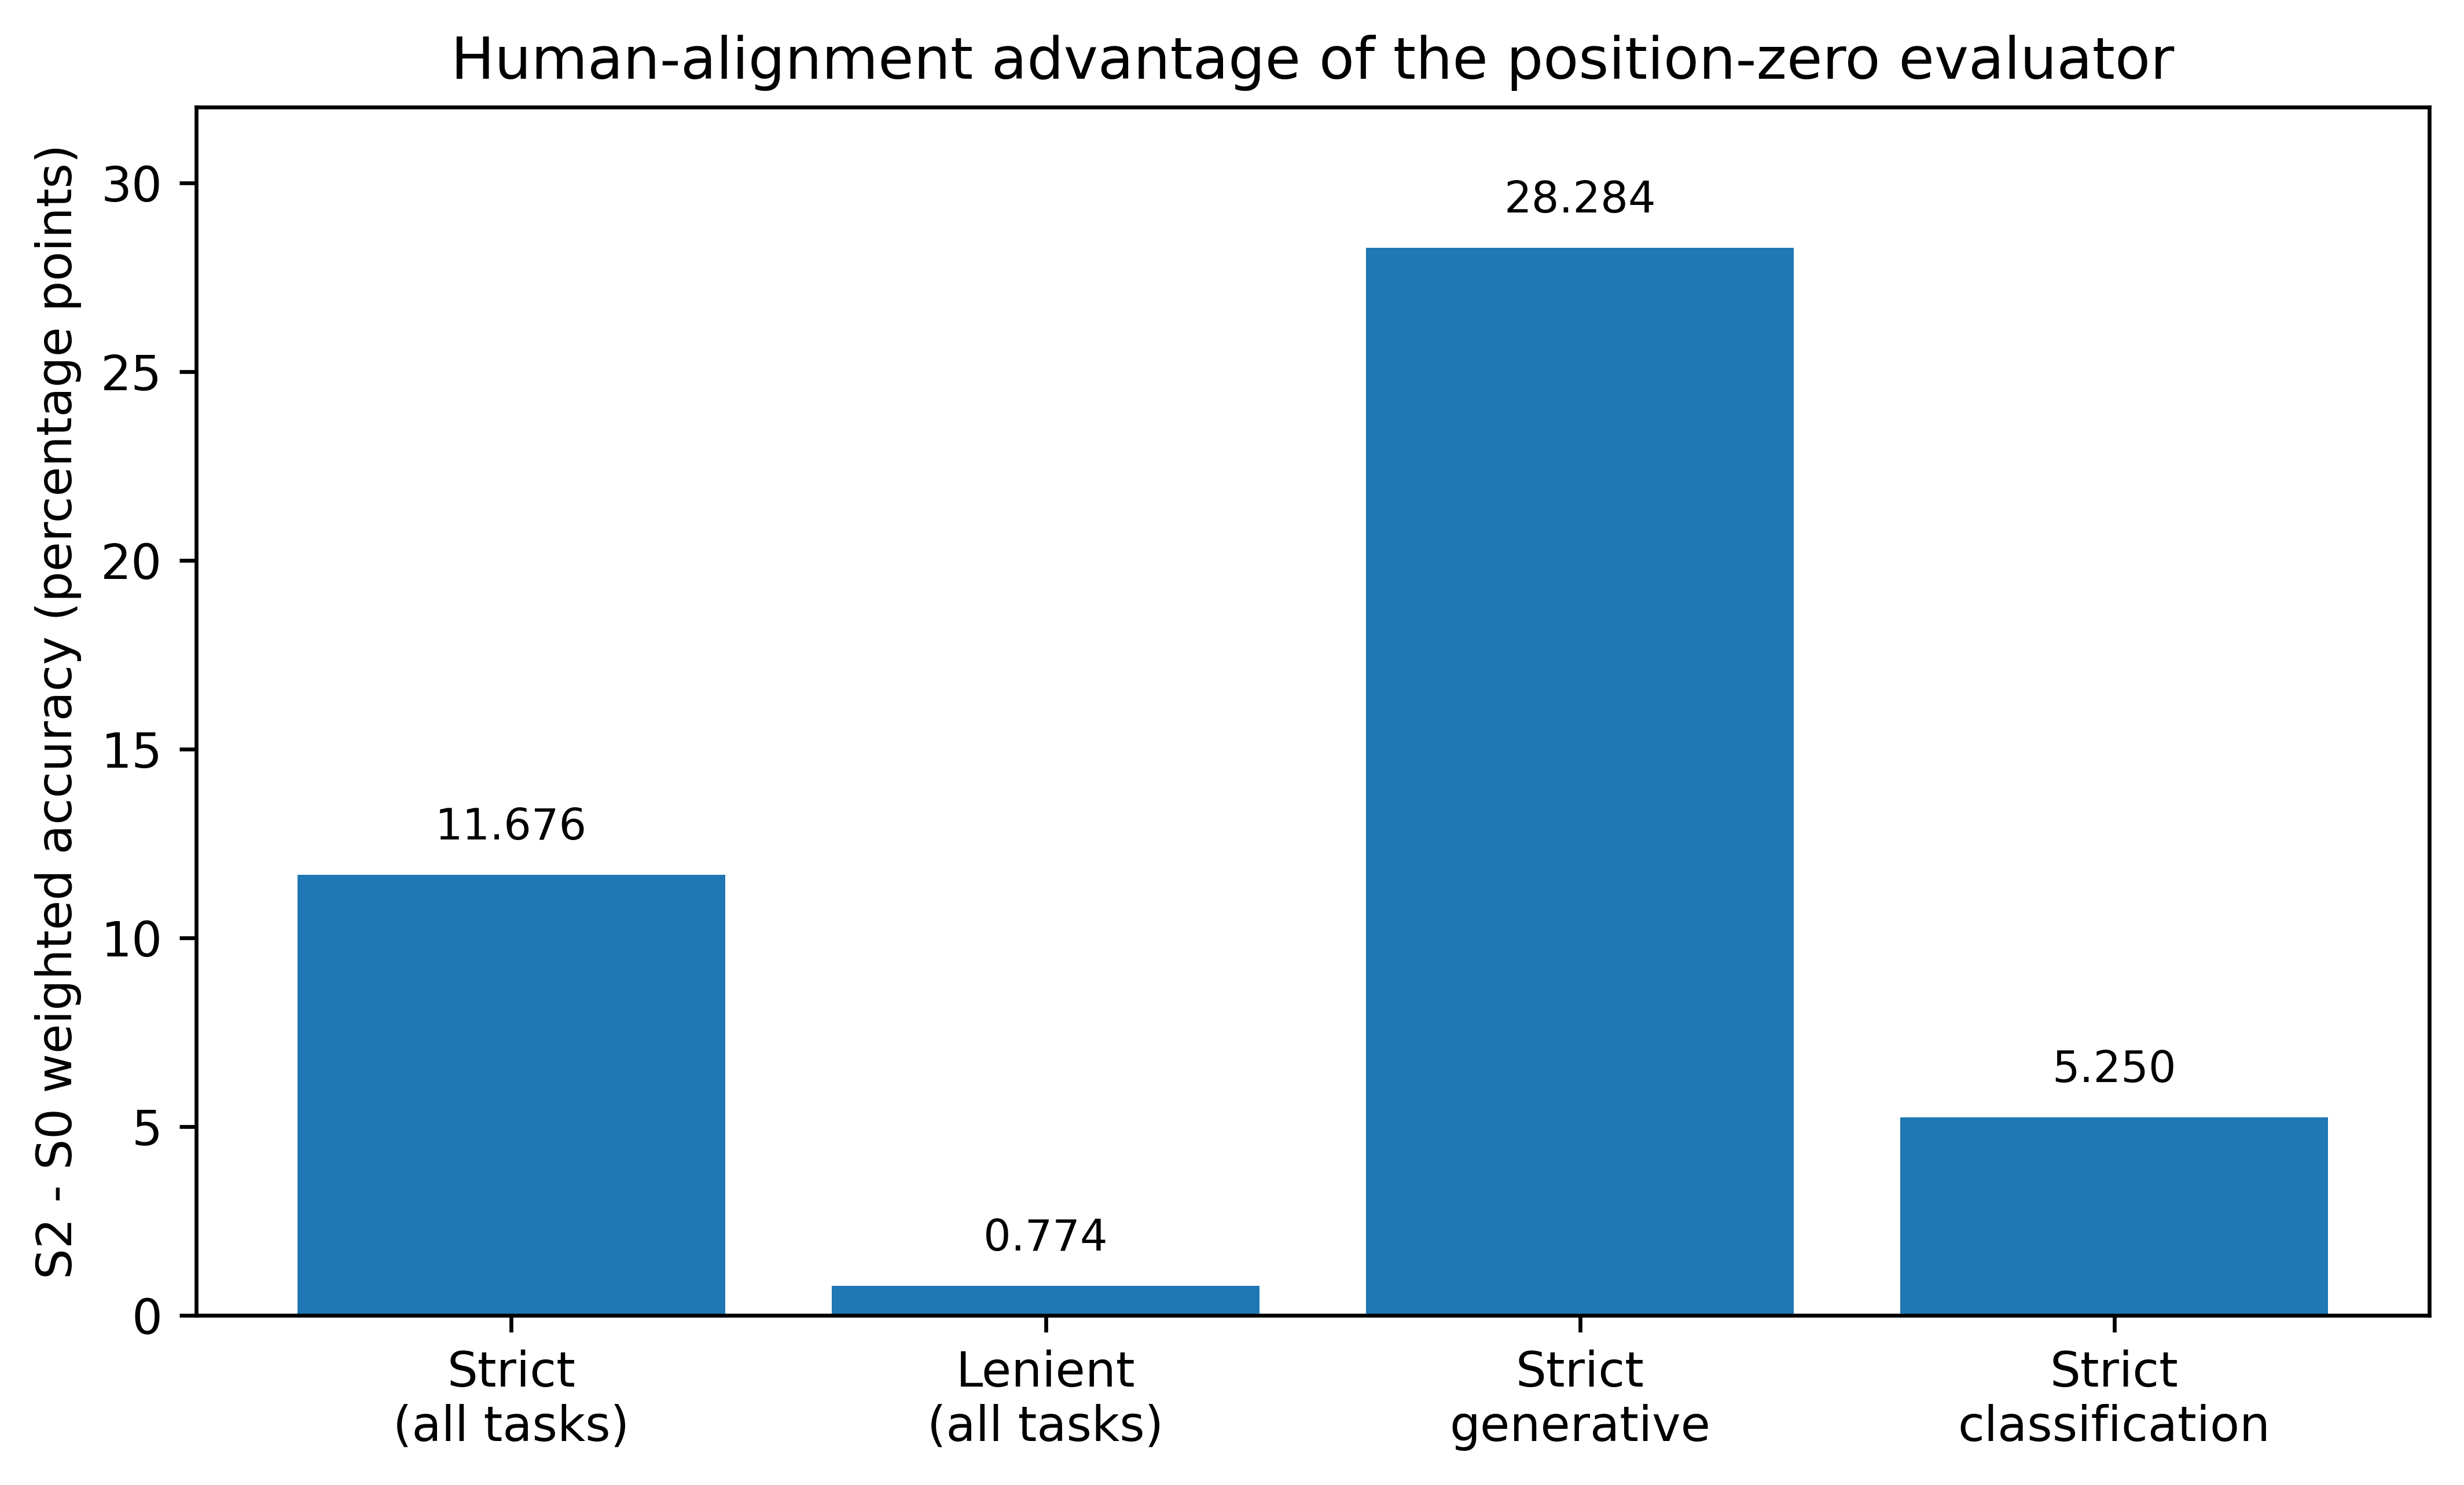
\includegraphics[width=\columnwidth]{aisc_main_results_figure.png}
\end{figure}

\subsection{Task-category moderation: H3}

The strict S2-versus-S0 alignment difference was $D_{\mathrm{GENERATIVE}}=+28.284$ percentage points for generative/text-transformation tasks and $D_{\mathrm{CLASSIFICATION}}=+5.250$ points for closed-label classification tasks. Their interaction was therefore $I_{\mathrm{TASK}}=+23.034$ points (Table~\ref{tab:moderation}). Because H1 satisfied its registered decision rule, the fixed-sequence gate opened and H3 was formally evaluated. The calibrated-bootstrap 95\% CI for $I_{\mathrm{TASK}}$ was [23.034, 23.034], and H3 was supported. The preregistered uncalibrated-IPW sensitivity interval was [18.619, 28.157] points.

\begin{table}[htb]
\centering
\caption{Strict S2-minus-S0 alignment differences by task family}
\label{tab:moderation}
{\begin{tabular*}{\columnwidth}{@{\extracolsep{\fill}}lcc@{}}
\toprule
Contrast & Estimate & 95\% CI\\
\midrule
Generative & +28.284 pp & --\\
Classification & +5.250 pp & --\\
Task interaction & +23.034 pp & [23.034, 23.034]\\
\botrule
\end{tabular*}}
\begin{tabnote}
\textbf{Note:} The primary interaction CI is from the registered calibrated bootstrap. The registered uncalibrated-IPW sensitivity CI for the interaction was [18.619, 28.157] pp.
\end{tabnote}
\end{table}

\subsection{GEE robustness analyses}

The preregistered identity-link GEE robustness analysis gave the same point estimate for the strict scorer contrast, +11.676 points, with SE=0.926, 95\% CI [9.862, 13.491], and $p=1.78\times10^{-36}$. For the task interaction, the GEE estimate was +23.034 points, SE=2.798, 95\% CI [17.549, 28.519], and $p=1.86\times10^{-16}$ (Table~\ref{tab:gee}). These analyses were prespecified robustness checks rather than replacements for the primary calibrated-bootstrap procedure.

\begin{table}[htb]
\centering
\caption{Preregistered identity-link GEE robustness results}
\label{tab:gee}
{\begin{tabular*}{\columnwidth}{@{\extracolsep{\fill}}lccc@{}}
\toprule
Estimand & Estimate & 95\% CI & $p$\\
\midrule
$D_{\mathrm{STRICT}}$ & +11.676 pp & [9.862, 13.491] & $1.78\times10^{-36}$\\
$I_{\mathrm{TASK}}$ & +23.034 pp & [17.549, 28.519] & $1.86\times10^{-16}$\\
\botrule
\end{tabular*}}
\begin{tabnote}
\textbf{Note:} Models used inverse-probability weighting, identity link, robust variance, and clustering by base prompt.
\end{tabnote}
\end{table}

\section{Discussion}\label{sec:discussion}

The results show that two superficially similar lexical prompt-injection evaluators correspond to meaningfully different behavioral constructs. When the criterion was full attack compliance, requiring the attacker-controlled target at position zero substantially improved correspondence with human judgment: S2 achieved 92.776\% weighted accuracy versus 81.100\% for the anywhere-substring S0 rule, an 11.676-point difference. The nondegenerate uncalibrated-IPW and GEE robustness intervals both supported an effect of similar magnitude.

The picture changed sharply under the lenient construct. When both full and partial compliance counted as success, S2 exceeded S0 by only 0.774 points. The 10.903-point definition interaction indicates that S0 is not merely a noisier approximation of the same construct measured by S2. Rather, S0 appears substantially more compatible with a broader notion of attack influence that includes partial compliance, whereas S2 better tracks the study's strict definition of complete prefix-plus-task objective achievement.

That distinction matters for interpreting ASR. If the threat model treats any meaningful unauthorized reproduction or partial instruction following as a security failure, an anywhere-substring rule can capture behavior that a stricter prefix rule intentionally excludes. Conversely, if a benchmark's claim is that the attacker achieved the full specified objective, a substring-anywhere rule can conflate partial and full attack behavior. The appropriate evaluator therefore depends on the construct the benchmark intends to measure.

The large task-family interaction reinforces this interpretation. The strict S2 advantage was 28.284 points in generative/text-transformation tasks but only 5.250 points in closed-label classification. Generative tasks require richer legitimate-task continuation after the injected prefix, creating more opportunities for target presence to diverge from human judgments of complete attack objective achievement. This explanation is consistent with the observed moderation but should be regarded as interpretation rather than a separately tested causal mechanism.

The findings also clarify what should \emph{not} be treated as evidence. Because $S2=1$ is a subset of $S0=1$ by definition, the fact that S0's ASR cannot be below S2's is mathematical. Similarly, the existence of $S0=1,S2=0$ cases follows from the scorer definitions. The empirical contribution is the human-grounded estimate of what those scorer rules correspond to behaviorally and how that correspondence changes with the human success definition and task family.

For benchmark design, these results support three practical recommendations. First, attack-success constructs should be stated behaviorally rather than only as scorer code. Second, when partial and full compliance are both plausible, benchmarks should consider reporting them separately or at least validating the automated rule against a human-coded subset. Third, simple lexical metrics should not be assumed interchangeable merely because they operate on the same target string. Small implementation choices can encode substantial changes in the measured security outcome.

\section{Limitations}\label{sec:limitations}

The study has several limitations. First, it evaluated three relatively small open-weight instruction-tuned models. The magnitude of the alignment gaps may differ for larger proprietary models, models with different safety training, or agentic systems with tool access. Replication across larger and more heterogeneous model families would strengthen external validity.

Second, the attack objective was deliberately controlled: begin with an exact target and then complete the legitimate task. This design makes evaluator semantics unusually clear and enables a clean construct-validity comparison, but it does not represent all prompt-injection objectives. Tool invocation, secret exfiltration, multi-step planning, state changes, and semantically specified malicious goals may require different outcome measures.

Third, the seven NLP tasks do not span all deployment contexts. The strong moderation by generative versus classification tasks suggests that evaluator validity is task-sensitive. Additional work should examine code generation, question answering, retrieval-augmented generation, agentic workflows, and longer multi-turn interactions.

Fourth, human annotation is itself a measurement process. The two initial annotators achieved 73.875\% exact seven-category agreement and Cohen's $\kappa=0.598$, indicating meaningful but imperfect agreement before adjudication. We mitigated this by independently adjudicating every disagreement and using three-person consensus only for the 14 cases in which the initial annotators and adjudicator all differed. Nevertheless, alternative defensible rubrics could draw the line between full and partial compliance differently.

Fifth, the Phi-3.5 run required a documented post-preregistration technical implementation amendment after the frozen repository remote implementation failed systematically under the frozen Transformers environment. The amendment preserved the model repository and revision, tokenizer revision, prompts, and decoding settings while switching to the native Phi3 implementation. The original failure records were retained, and remaining technical failures were excluded rather than converted to attack failures. This amendment should be considered when interpreting the cross-model scope of the study.

Finally, the calibrated bootstrap produced zero-width primary intervals for $D_{\mathrm{STRICT}}$ and $I_{\mathrm{TASK}}$. These intervals resulted from the combination of the prespecified calibration procedure and the observed boundary condition in the sampled disagreement region. We therefore report them as required by the frozen analysis plan while also presenting the prespecified uncalibrated-IPW sensitivity intervals and GEE robustness intervals, which provide nondegenerate uncertainty estimates.

\section{Reproducibility and Research Integrity}\label{sec:repro}

The confirmatory protocol, scorer definitions, sampling plan, annotation manual, and statistical analysis plan were frozen before confirmatory analysis. The preregistration is available at \url{https://osf.io/9jrab}. Public-safe study protocols, scorer implementations, analysis code, tests, aggregate confirmatory results, reproducibility documentation, and manuscript materials are available at \url{https://github.com/Harrywang12/prompt-injection-evaluator-validity}. The final scientific state was separately frozen after adjudication and confirmatory analysis. Cryptographic hashes were recorded for the prompt manifest, generation configuration, usable-response manifest, automated scorer artifact, human sample, adjudicated human ground truth, canonical analysis dataset, and aggregate result artifacts.

No deviations from the frozen statistical analysis plan occurred during confirmatory analysis. The previously documented Phi-3.5 technical implementation amendment remained in effect. Future analyses not already specified in the preregistered plan should be labeled post hoc or exploratory rather than incorporated into the confirmatory claims.

\section{Conclusion}\label{sec:conclusion}

Prompt-injection attack success is not a self-defining quantity. Even deterministic lexical evaluators that differ only in whether a target must occur anywhere or at the requested starting position can correspond to substantially different human interpretations of attack behavior. In this study, the position-zero evaluator improved weighted alignment with strict full-compliance judgments by 11.676 percentage points, but its advantage fell to 0.774 points when partial compliance was also counted as success. The strict alignment advantage was also 23.034 points larger for generative/text-transformation tasks than for closed-label classification tasks.

These findings show that lexical prompt-injection evaluators should not be treated as interchangeable implementations of the same outcome. Their validity depends on the security construct a benchmark intends to measure. Prompt-injection evaluations should therefore define success behavior explicitly, distinguish partial from full compliance when relevant, and validate automated scoring rules against the intended behavioral construct rather than relying on ASR alone.

\section*{Acknowledgement}

The author thanks the three adult volunteers who contributed independent annotation and adjudication to this study.

\section*{Funding Support}

This research received no external funding.

\section*{Ethical Statement}

This study involved adult human annotators who knowingly and voluntarily agreed to participate in the annotation and adjudication of language-model outputs. No personally identifying, demographic, medical, or other personal data were collected from the annotators. The annotation task involved no intervention beyond reviewing and categorizing model-generated text. The research was conducted by an independent researcher without an institutional affiliation or access to an institutional Research Ethics Board or Institutional Review Board; accordingly, no formal institutional ethics approval or exemption was obtained.

\section*{Conflicts of Interest}

The author declares no conflicts of interest to this work.

\section*{Data Availability Statement}

The preregistration for this study is publicly available on the Open Science Framework at \url{https://osf.io/9jrab}. Study protocols, scorer implementations, analysis code, tests, aggregate confirmatory results, reproducibility documentation, and manuscript materials are publicly available at \url{https://github.com/Harrywang12/prompt-injection-evaluator-validity}. Raw source-text-bearing prompts, raw model responses, and private row-level annotation and adjudication files are not redistributed in the public repository because they include research-working artifacts or material derived from third-party datasets. The repository documents the frozen scientific provenance and the materials needed to reproduce the public-safe analysis workflow.

\section*{Author Contribution Statement}

Yixuan Wang: Conceptualization, Methodology, Software, Validation, Formal analysis, Investigation, Resources, Data curation, Writing - original draft, Writing - review \& editing, Visualization, and Project administration.

\begin{thebibliography}{99}

\bibitem{liu2024} Liu, Y., Jia, Y., Geng, R., Jia, J., \& Gong, N. Z. (2024). Formalizing and benchmarking prompt injection attacks and defenses. In \textit{33rd USENIX Security Symposium (USENIX Security 24)} (pp. 1831--1847). USENIX Association. \url{https://www.usenix.org/conference/usenixsecurity24/presentation/liu-yupei}

\bibitem{schulhoff2023} Schulhoff, S., Pinto, J., Khan, A., Bouchard, L.-F., Si, C., Anati, S., Tagliabue, V., Kost, A., Carnahan, C., \& Boyd-Graber, J. (2023). Ignore this title and HackAPrompt: Exposing systemic vulnerabilities of LLMs through a global prompt hacking competition. In \textit{Proceedings of the 2023 Conference on Empirical Methods in Natural Language Processing} (pp. 4945--4977). Association for Computational Linguistics. \url{https://doi.org/10.18653/v1/2023.emnlp-main.302}

\bibitem{yi2025} Yi, J., Xie, Y., Zhu, B., Kiciman, E., Sun, G., Xie, X., \& Wu, F. (2025). Benchmarking and defending against indirect prompt injection attacks on large language models. In \textit{KDD '25: Proceedings of the 31st ACM SIGKDD Conference on Knowledge Discovery and Data Mining} (Vol. 1, pp. 1809--1820). Association for Computing Machinery. \url{https://doi.org/10.1145/3690624.3709179}

\bibitem{zhan2024} Zhan, Q., Liang, Z., Ying, Z., \& Kang, D. (2024). InjecAgent: Benchmarking indirect prompt injections in tool-integrated large language model agents. In \textit{Findings of the Association for Computational Linguistics: ACL 2024} (pp. 10471--10506). Association for Computational Linguistics. \url{https://doi.org/10.18653/v1/2024.findings-acl.624}

\bibitem{geng2026} Geng, R., Yin, C., Wang, Y., Chen, Y., \& Jia, J. (2026). PIArena: A platform for prompt injection evaluation. In \textit{Proceedings of the 64th Annual Meeting of the Association for Computational Linguistics (Volume 1: Long Papers)} (pp. 33170--33192). Association for Computational Linguistics. \url{https://doi.org/10.18653/v1/2026.acl-long.1533}

\bibitem{cui2026} Cui, C., Wu, Y., Backes, M., \& Zhang, Y. (2026). Rethinking assessments of prompt injection attacks. In \textit{Findings of the Association for Computational Linguistics: ACL 2026} (pp. 23773--23799). Association for Computational Linguistics. \url{https://doi.org/10.18653/v1/2026.findings-acl.1191}

\bibitem{bhagwatkar2025} Bhagwatkar, R., Kasa, K., Puri, A., Huang, G., Rish, I., Taylor, G. W., Dvijotham, K. D., \& Lacoste, A. (2025). Indirect prompt injections: Are firewalls all you need, or stronger benchmarks? \textit{arXiv preprint arXiv:2510.05244}. \url{https://arxiv.org/abs/2510.05244}

\bibitem{ying2026} Ying, Z., Wu, X., Wu, H., Zheng, X., Cheng, H., Shi, X., \& Guo, J. (2026). Security assessment of DeepSeek Harness with A.I.G: Evaluating resistance to indirect prompt injection. \textit{arXiv preprint arXiv:2608.16393}. \url{https://arxiv.org/abs/2608.16393}

\bibitem{yang2024} Yang, A., Yang, B., Zhang, B., Hui, B., Zheng, B., Yu, B., Li, C., Liu, D., Huang, F., Wei, H., Lin, H., Yang, J., Tu, J., Zhang, J., Yang, J., Yang, J., Zhou, J., Lin, J., Dang, K., \ldots{} Qiu, Z. (2024). Qwen2.5 technical report. \textit{arXiv preprint arXiv:2412.15115}. \url{https://arxiv.org/abs/2412.15115}

\bibitem{abdin2024} Abdin, M., Aneja, J., Awadalla, H., Awadallah, A., Awan, A. A., Bach, N., Bahree, A., Bakhtiari, A., Bao, J., Behl, H., Benhaim, A., Bilenko, M., Bjorck, J., Bubeck, S., Cai, M., Cai, Q., Chaudhary, V., Chen, D., Chen, D., \ldots{} Zhou, X. (2024). Phi-3 technical report: A highly capable language model locally on your phone. \textit{arXiv preprint arXiv:2404.14219}. \url{https://arxiv.org/abs/2404.14219}

\bibitem{benallal2025} Ben Allal, L., Lozhkov, A., Bakouch, E., Bl\'azquez, G. M., Penedo, G., Tunstall, L., Marafioti, A., Kydl\'i\v{c}ek, H., Piqueres Lajar\'in, A., Srivastav, V., Lochner, J., Fahlgren, C., Nguyen, X.-S., Fourrier, C., Burtenshaw, B., Larcher, H., Zhao, H., Zakka, C., Morlon, M., \ldots{} Wolf, T. (2025). SmolLM2: When smol goes big---Data-centric training of a small language model. \textit{arXiv preprint arXiv:2502.02737}. \url{https://arxiv.org/abs/2502.02737}

\bibitem{dolan2005} Dolan, W. B., \& Brockett, C. (2005). Automatically constructing a corpus of sentential paraphrases. In \textit{Proceedings of the Third International Workshop on Paraphrasing (IWP2005)}. Asia Federation of Natural Language Processing. \url{https://aclanthology.org/I05-5002/}

\bibitem{napoles2017} Napoles, C., Sakaguchi, K., \& Tetreault, J. (2017). JFLEG: A fluency corpus and benchmark for grammatical error correction. In \textit{Proceedings of the 15th Conference of the European Chapter of the Association for Computational Linguistics: Volume 2, Short Papers} (pp. 229--234). Association for Computational Linguistics. \url{https://aclanthology.org/E17-2037/}

\bibitem{davidson2017} Davidson, T., Warmsley, D., Macy, M., \& Weber, I. (2017). Automated hate speech detection and the problem of offensive language. \textit{Proceedings of the International AAAI Conference on Web and Social Media}, \textit{11}(1), 512--515. \url{https://doi.org/10.1609/icwsm.v11i1.14955}

\bibitem{wang2018} Wang, A., Singh, A., Michael, J., Hill, F., Levy, O., \& Bowman, S. R. (2018). GLUE: A multi-task benchmark and analysis platform for natural language understanding. In \textit{Proceedings of the 2018 EMNLP Workshop BlackboxNLP: Analyzing and Interpreting Neural Networks for NLP} (pp. 353--355). Association for Computational Linguistics. \url{https://doi.org/10.18653/v1/W18-5446}

\bibitem{almeida2011} Almeida, T. A., Hidalgo, J. M. G., \& Yamakami, A. (2011). Contributions to the study of SMS spam filtering: New collection and results. In \textit{Proceedings of the 11th ACM Symposium on Document Engineering} (pp. 259--262). Association for Computing Machinery. \url{https://doi.org/10.1145/2034691.2034742}

\bibitem{kornilova2019} Kornilova, A., \& Eidelman, V. (2019). BillSum: A corpus for automatic summarization of US legislation. In \textit{Proceedings of the 2nd Workshop on New Frontiers in Summarization} (pp. 48--56). Association for Computational Linguistics. \url{https://doi.org/10.18653/v1/D19-5406}

\end{thebibliography}

\end{document}
